%%=====================================================================
%%  A Hybrid Zero Trust Architecture for Non-Interactive Authentication
%%  Integrating Hardware Trust Anchors with Software-Defined Secret
%%  Management in Infrastructure as Code
%%
%%  Revised manuscript aligned with the public reference implementation
%%  (https://github.com/juarez1972/app-tpm): Twingate ZTNA, TOTP-over-TPM
%%  IoT agent, Vault TPM auto-unseal, and LLM red-team pentest module.
%%
%%  REVISION (July 2026): new Background and Related Work section;
%%  expanded bibliography (57 entries);
%%  Threats to Validity subsection; hardware side-channel discussion;
%%  continuous-attestation roadmap. Bibliography: references.bib.
%%
%%  Compile with:  pdflatex hybrid_zt_nia.tex  (x2, for cross-refs)
%%  Requires the IEEEtran document class (texlive-publishers).
%%=====================================================================
\documentclass[journal]{IEEEtran}
% Standard IEEE journal format: 10pt, two-column, final layout.
% Wide floats (tables/figures) use the starred environments (table*/figure*).

\usepackage{cite}
\usepackage{seqsplit}   % allow long monospace paths/identifiers to wrap
\usepackage{amsmath,amssymb,amsfonts}
\usepackage{algorithmic}
\usepackage{graphicx}
\usepackage{textcomp}
\usepackage{xcolor}
\usepackage{booktabs}
\usepackage{array}
\usepackage{url}
\usepackage{listings}
\usepackage{tikz}
\usetikzlibrary{arrows.meta,positioning,fit,backgrounds,calc,shapes.geometric}
\usepackage{stfloats}   %% allow double-column floats at top/bottom of page
\usepackage{afterpage}  %% release a float at the next page break (top of p.2)
\usepackage{hyperref}
\hypersetup{colorlinks=true,linkcolor=blue,citecolor=blue,urlcolor=blue}

\lstset{
  basicstyle=\ttfamily\footnotesize,
  breaklines=true,
  columns=fullflexible,
  frame=single,
  captionpos=b,
  language=Python
}

% Breakable typewriter macro: long paths/identifiers may wrap in the narrow
% two-column measure (allows breaks after common separators, no hyphen added).
\newcommand{\ttcmd}[1]{\texttt{\seqsplit{#1}}}

\begin{document}

\title{A Hybrid Zero Trust Architecture for Non-Interactive Authentication:
Integrating Hardware Trust Anchors with Software-Defined Secret Management
in Infrastructure as Code}

\author{
\IEEEauthorblockN{Juarez de Oliveira, Juliano S. Langaro, Fellipe M. Veiga, Altair O. Santin, and Eduardo K. Viegas}
\IEEEauthorblockA{Graduate Program in Computer Science (PPGIa) | Pontifical Catholic University of Parana (PUCPR), Brazil\\
\{juarez.oliveira, juliano.langaro, fellipe.veiga, altair.santin, eduardo.viegas\}@ppgia.pucpr.br}%
\thanks{This work was partially sponsored by CNPq under grants
307706/2025-7 and 407879/2023-4.}%
\thanks{Manuscript revised July~22, 2026. The reference implementation is
publicly available at \url{https://github.com/juarez1972/app-tpm}.}}

\markboth{IEEE Transactions on Information Forensics and Security}%
{Oliveira \MakeLowercase{\textit{et al.}}: Hybrid ZT Architecture for Non-Interactive Authentication}

\maketitle

\begin{abstract}
Non-Interactive Authentication (nIA)---the machine-to-machine authentication
that underpins Infrastructure as Code (IaC) pipelines and unattended
Internet-of-Things (IoT) fleets---is chronically undermined by the
\emph{Secret Zero} problem: a long-lived credential must be planted somewhere
in software to bootstrap every other secret, and that credential is
extractable under operating-system compromise (MITRE ATT\&CK T1003).
This paper presents a hybrid Zero Trust architecture that anchors secret
management in \emph{hardware trust anchors} (TPM~2.0, with an upgrade path to
Intel SGX and TDX), delegates HashiCorp Vault auto-unseal to a physical TPM,
and confines every credential inside an identity-based network perimeter
(ZTNA) so that intercepted secrets cannot be replayed outside their network
context. We describe a working reference implementation, publicly released,
whose IoT agent seals a per-device \emph{time-based one-time password} (TOTP,
RFC~6238) seed inside the device TPM while registering the same seed in the
server's Vault, so the plaintext seed never touches disk on either side; the
TOTP HMAC is delegated to the TPM so the key never leaves the silicon, and the
code itself is transmitted only inside an \emph{HMAC envelope} so it is never
sent in the clear. We
evaluate the design along three axes: (i) \emph{provisioning time} for the full
infrastructure, (ii) \emph{secret-retrieval latency} on the hot path, and
(iii) resistance to an on-premises Large-Language-Model (LLM) red-team mapped
to MITRE ATT\&CK. We further contribute a \emph{proposed security-test suite}
that turns the ad-hoc red-team into a repeatable regression gate executed
after each \texttt{terraform apply}. Measured software-path costs (TOTP
generation and cached seed retrieval) are sub-25 microseconds; the hardware
path adds a bounded, single-digit-to-tens-of-milliseconds overhead while
reducing Vault recovery time objective (RTO) from minutes to milliseconds.
Results are reported as indicative estimates backed by prototype measurements;
production-scale empirical validation remains future work.
\end{abstract}

\begin{IEEEkeywords}
Zero Trust, Trusted Platform Module, HashiCorp Vault, non-interactive
authentication, Infrastructure as Code, MITRE ATT\&CK, IoT security,
confidential computing, TOTP, LLM red-teaming.
\end{IEEEkeywords}

%%---------------------------------------------------------------------
\section{Introduction}
%%---------------------------------------------------------------------

%%------------------- Architecture figure (TikZ), pinned to top of p.2 -------------------
%% Released at the first page break via \afterpage so the double-column
%% float lands at the TOP of page 2 rather than drifting into the body flow.
\afterpage{%
\begin{figure*}[t]
\centering
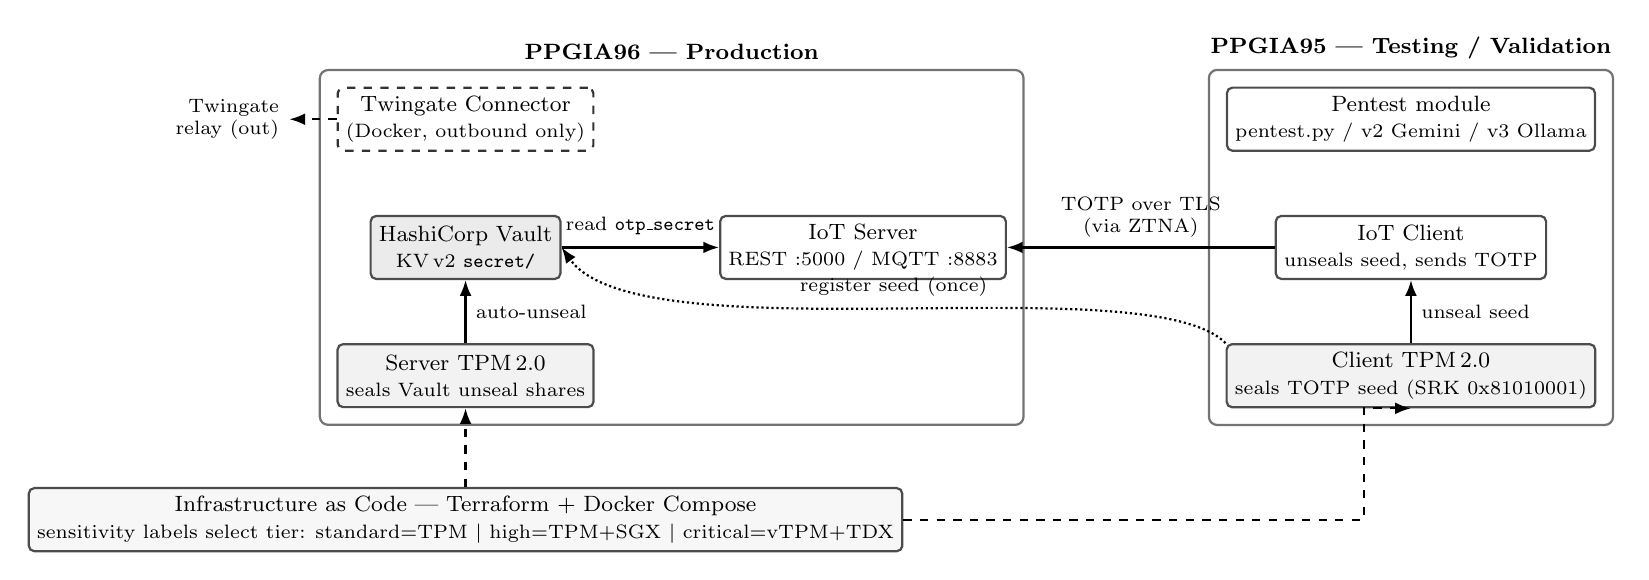
\begin{tikzpicture}[
  font=\footnotesize,
  node distance=6mm,
  box/.style={rectangle,rounded corners=2pt,draw=black!70,thick,
              align=center,minimum height=8mm,inner sep=3pt,fill=white},
  hw/.style={box,fill=black!5},
  vault/.style={box,fill=black!8},
  ztna/.style={box,draw=black!80,dashed},
  layerlbl/.style={font=\footnotesize\bfseries,align=left},
  flow/.style={-{Latex[length=2mm]},thick},
  ctrl/.style={-{Latex[length=2mm]},thick,dashed},
  server/.style={rectangle,rounded corners=3pt,draw=black!55,thick,inner sep=6pt}
]

% ===================== PPGIA96 (production) =====================
% Layer 3 - ZTNA connector (top of production server)
\node[ztna] (conn) {Twingate Connector\\\scriptsize (Docker, outbound only)};
% Layer 2 - Vault
\node[vault,below=8mm of conn] (vault) {HashiCorp Vault\\\scriptsize KV\,v2 \texttt{secret/}};
\node[box,right=20mm of vault] (srv) {IoT Server\\\scriptsize REST :5000 / MQTT :8883};
% Layer 1 - TPM (server)
\node[hw,below=8mm of vault] (stpm) {Server TPM\,2.0\\\scriptsize seals Vault unseal shares};

\begin{scope}[on background layer]
  \node[server,fit=(conn)(vault)(srv)(stpm),
        label={[font=\footnotesize\bfseries]above:PPGIA96 --- Production}] (p96) {};
\end{scope}

% ===================== PPGIA95 (testing) =====================
\node[box,right=34mm of srv] (client) {IoT Client\\\scriptsize unseals seed, sends TOTP};
\node[hw,below=8mm of client] (ctpm) {Client TPM\,2.0\\\scriptsize seals TOTP seed (SRK 0x81010001)};
\node[box,above=8mm of client] (pentest) {Pentest module\\\scriptsize pentest.py / v2 Gemini / v3 Ollama};

\begin{scope}[on background layer]
  \node[server,fit=(client)(ctpm)(pentest),
        label={[font=\footnotesize\bfseries]above:PPGIA95 --- Testing / Validation}] (p95) {};
\end{scope}

% ===================== IaC layer (bottom, spanning) =====================
\node[box,fill=black!3,below=10mm of stpm,minimum width=52mm] (iac)
  {Infrastructure as Code --- Terraform + Docker Compose\\\scriptsize sensitivity labels select tier: standard=TPM $\vert$ high=TPM+SGX $\vert$ critical=vTPM+TDX};

% ===================== edges =====================
% provisioning: IaC drives both servers
\draw[ctrl] (iac.north) -- ++(0,4mm) -| (stpm.south);
\draw[ctrl] (iac.east) -| ($(ctpm.south)+(-6mm,0)$) -- (ctpm.south);
% server-side: TPM auto-unseal -> Vault
\draw[flow] (stpm) -- node[right,font=\scriptsize]{auto-unseal} (vault);
% server reads seed from Vault
\draw[flow] (vault) -- node[midway,above=1pt,font=\scriptsize]{read \texttt{otp\_secret}} (srv);
% client TPM -> client (unseal)
\draw[flow] (ctpm) -- node[right,font=\scriptsize]{unseal seed} (client);
% client -> server over ZTNA (the only path between servers)
\draw[flow] (client) -- node[above,font=\scriptsize,align=center]{TOTP over TLS\\(via ZTNA)} (srv);
% connector mediates: dashed boundary to relay
\draw[ctrl] (conn.west) -- ++(-6mm,0) node[left,font=\scriptsize,align=right]{Twingate\\relay (out)};
% provisioning registers seed in Vault (one-time)
\draw[flow,densely dotted] (ctpm.north west) .. controls +(-10mm,10mm) and +(10mm,-14mm) ..
     node[above,font=\scriptsize,pos=0.5]{register seed (once)} (vault.east);

\end{tikzpicture}
\caption{Hybrid Zero Trust architecture. \emph{Layer~1} (hardware root of trust)
seals credentials in the TPM on both hosts; \emph{Layer~2} (Vault) is
TPM-auto-unsealed and stores per-device OTP seeds; \emph{Layer~3} (ZTNA) exposes
services only through an outbound-only Twingate connector. The IoT seed is
sealed in the client TPM and registered once in the server Vault (dotted),
so the plaintext seed never touches disk; at run time the client sends a TOTP
over TLS through the ZTNA perimeter, and the server reads the matching seed
from Vault. Everything is provisioned by IaC, which also selects the protection
tier.}
\label{fig:arch}
\end{figure*}%
}

\IEEEPARstart{M}{odern} infrastructure is provisioned by code and operated by
machines. IaC engines apply changes without a human at the keyboard, and IoT
fleets authenticate to back-ends at boot with no operator present. This
\emph{non-interactive} setting removes the human factor that interactive
multi-factor authentication (MFA) relies on, and it forces a bootstrap
credential---the \emph{Secret Zero}---to live in software. Once an adversary
attains operating-system privileges, that credential and any secret it
unlocks become extractable (MITRE ATT\&CK T1003, OS Credential Dumping;
T1552, Unsecured Credentials).

Software-only secret managers such as HashiCorp Vault mitigate sprawl but do
not by themselves solve Secret Zero: Vault must itself be unsealed, and the
unseal material is the new Secret Zero. Prior work by Oliveira \emph{et al.}
\cite{oliveira2024} showed that a non-interactive one-time-password (OTP)
method materially raises the cost of Vault credential abuse; this paper
generalizes and hardens that line of work by moving the trust anchor into
silicon and enclosing the entire flow in an identity-based network perimeter.

\textbf{Contributions.} This revision consolidates and extends our earlier
results:
\begin{enumerate}
\item A three-layer \emph{hybrid} Zero Trust design that combines a hardware
root of trust (TPM~2.0, with SGX/TDX tiers), software-defined secret
management (Vault auto-unseal), and identity-based network access (ZTNA via a
Twingate connector deployed on-premises).
\item A hardware-anchored one-time-password scheme in which the shared seed is
sealed inside the TPM and is non-exportable, so credential theft requires
physical silicon tampering rather than a software read.
\item A protocol-agnostic, two-channel MFA model for unattended IoT that
operates over both REST/HTTPS and MQTT/TLS.
\item An IaC-driven tiered protection model (TPM / SGX / TDX) selected
automatically through Terraform sensitivity labels.
\item A reproducible, on-premises LLM adversary simulation mapped to MITRE
ATT\&CK, and---new in this revision---(v)~a \emph{provisioning-time and
secret-retrieval-latency} characterization of the running prototype,
(vi)~a \emph{proposed security-test suite} that converts the red-team into a
post-deployment regression gate, and (vii)~an \emph{on-the-wire HMAC envelope}
that obfuscates the transmitted one-time password so the code is never sent in
the clear (Section~\ref{sec:envelope}).
\end{enumerate}

The remainder of the paper is organized as follows.
Section~\ref{sec:related} reviews background and related work.
Section~\ref{sec:threat} states the threat model.
Section~\ref{sec:arch} describes the architecture and its mapping to the public
reference implementation.
Section~\ref{sec:impl} details the implementation, including the exact
mechanism by which the OTP seed is sealed and retrieved.
Section~\ref{sec:tests} proposes the security-test suite.
Section~\ref{sec:eval} reports the simulation-based evaluation, provisioning
time, and secret-retrieval latency.
Section~\ref{sec:disc} discusses limitations, threats to validity, and an
additional operational point (supply-chain and reproducibility).
Section~\ref{sec:concl} concludes.

%%---------------------------------------------------------------------
\section{Background and Related Work}\label{sec:related}
%%---------------------------------------------------------------------

\subsection{Zero Trust Architectures}
Zero Trust replaces implicit network trust with per-request, identity-centric
authorization---a model pioneered by Google's BeyondCorp initiative
\cite{ward2014beyondcorp}, codified by NIST SP~800-207 \cite{nist800207}, and
recently complemented by the practical implementation guidance of NIST
SP~1800-35 \cite{nist1800_35}. Comprehensive surveys chart the maturation of
the model and its open challenges \cite{syed2022ztasurvey,he2022ztasurvey,
gambo2025ztaslr}, the difficulties of migrating legacy enterprises
\cite{teerakanok2021}, and its instantiation in network-centric and
IoT/6G-centric scenarios \cite{dhiman2024zerotrust,nahar2024zta6g}. Our work
follows this line but targets the \emph{non-interactive} corner case, where
neither interactive MFA nor user-driven posture checks are available.

\subsection{Secret Management and the Secret Zero Problem}
Empirical studies quantify how often static credentials leak from software
artifacts: Meli \emph{et al.} found secrets leaking from over $100{,}000$
public GitHub repositories, with thousands of new leaks every day
\cite{meli2019git}; automated detectors confirm the prevalence of plaintext
passwords in public repositories \cite{feng2022password}, and curated corpora
such as SecretBench \cite{basak2023secretbench} enable systematic study of the
phenomenon. Practitioner-focused work catalogs secret-management practices and
their pitfalls in software artifacts and IaC
\cite{basak2022,rahman2021,patel2025}, and zero-trust CI/CD frameworks address
the multi-tenant pipeline setting \cite{anuganti2025}. Software vaults
\cite{hashivault2024} centralize secrets but leave the bootstrap
credential---Secret Zero---unsolved \cite{oliveira2024}. A complementary
industry answer is federated \emph{workload identity} (SPIFFE/SPIRE), which
replaces static secrets with attested, short-lived identities in CI/CD
pipelines \cite{avirneni2025spiffe} and agentic AI ecosystems
\cite{pappu2025spiffeai}. These frameworks, however, root trust in
platform-level assertions; we complement them by binding the identity seed to
a \emph{discrete hardware anchor}, which extends the guarantee to
resource-constrained IoT endpoints at the edge.

\subsection{Hardware Trust Anchors and Remote Attestation}
TPM-based roots of trust are standardized by the TCG \cite{tcg2019} and have
been used to establish trust domains in IoT deployments
\cite{faisal2020tpmiot,furtak2019securedomain}. TEEs strengthen the software
side: SGX enclaves \cite{costan2016} run unmodified applications through
library OSes such as Gramine \cite{tsai2017graphene}, and confidential VMs
based on Intel TDX \cite{cheng2023} are served by slim guest kernels such as
Gramine-TDX \cite{kuvaiskii2024gramine}, with independently benchmarked
performance envelopes \cite{coppolino2025}. Attestation of such anchors is
being standardized by the IETF RATS architecture \cite{rfc9334} and realized
by systems work on universal cloud/edge attestation \cite{ott2023universal},
TEE attestation mechanisms \cite{menetrey2022attestation}, ephemeral vTPMs
for confidential VMs \cite{narayanan2023vtpm}, and production-grade continuous
attestation with Keylime \cite{ruffin2025keylime}; recent efforts extend this
to attested Kubernetes workers \cite{thijsman2024attestedk8s}, 5G network
functions \cite{emran2025vnf}, and post-quantum IoT settings
\cite{eckel2025pqattest}. Our design currently uses the TPM for sealing and
keyed hashing, and SGX/TDX for isolation; integrating standards-based
continuous attestation is a natural evolution discussed in
Section~\ref{sec:disc}.

\subsection{Attacks on Trust Anchors}
Hardware anchors are not unassailable. TPM-FAIL recovered ECDSA private keys
from CC-certified TPMs through remote timing side channels
\cite{moghimi2020tpmfail}; cold-boot attacks recover keys from residual DRAM
\cite{halderman2008}; and transient-execution attacks such as Foreshadow
extracted SGX enclave secrets \cite{vanbulck2018foreshadow}.
Section~\ref{sec:threat} scopes physical and microarchitectural vectors out of
our software-adversary model, and Section~\ref{sec:disc} argues that our
primitive choices (TPM sealing and keyed hashing, rather than TPM-resident
ECDSA signing) reduce the surface exposed to the timing channels exploited by
TPM-FAIL.

\subsection{OTP-Based Authentication and IoT Transport Security}
HOTP/TOTP \cite{rfc4226,rfc6238}, built on HMAC \cite{rfc2104}, remain the
reference one-time-password constructions; our earlier work adapted them to
non-interactive Vault authentication \cite{oliveira2024}. On the transport
side, a large-scale analysis of real-world backends speaking IoT protocols
found widespread insecure MQTT deployments where TLS terminates at
intermediaries \cite{tagliaro2024backends}---precisely the exposure our
on-the-wire HMAC envelope addresses (Section~\ref{sec:envelope})---and
contemporary work explores stateful MQTT authentication with LLM-based
intrusion detection \cite{jamil2026mqtt}.

\subsection{LLM-Driven Offensive Security}
Autonomous LLM penetration testing emerged with PentestGPT \cite{pentestgpt},
early feasibility studies \cite{happe2023}, and AutoAttacker
\cite{autoattacker}. The line has since matured into autonomous privilege
escalation agents \cite{happe2025llmhackers}, end-to-end frameworks such as
HackSynth \cite{muzsai2024hacksynth} and the multi-agent VulnBot
\cite{kong2025vulnbot}, and dedicated benchmarks including AutoPenBench
\cite{gioacchini2024autopenbench} and CyberSecEval~2
\cite{bhatt2024cyberseceval2}. These works provide the methodological backdrop
for our regression-style, MITRE-mapped red-team (Sections~\ref{sec:tests}
and~\ref{sec:eval}).

%%---------------------------------------------------------------------
\section{Threat Model}\label{sec:threat}
%%---------------------------------------------------------------------
We assume a \emph{root-level software adversary}: an attacker who has achieved
privileged code execution on a host but who cannot physically decap or
glitch the TPM silicon. The adversary's goals and the corresponding MITRE
ATT\&CK techniques \cite{mitre2024} are:
\begin{itemize}
\item \textbf{Credential extraction} --- reading secrets from memory, disk, or
process space (T1003 OS Credential Dumping; T1552 Unsecured Credentials).
\item \textbf{Network interception} --- passively capturing OTP codes or
tokens in transit (T1040 Network Sniffing).
\item \textbf{Replay / token reuse} --- re-presenting a captured OTP or session
token (T1550 Use Alternate Authentication Material; T1078 Valid Accounts).
\item \textbf{Privilege escalation} --- abusing a foothold to reach a
higher-value service (T1068 Exploitation for Privilege Escalation;
tactic TA0004).
\item \textbf{Lateral movement} --- pivoting from a compromised host to another
(T1021 Remote Services; tactic TA0008).
\end{itemize}
Physical and microarchitectural attacks against the trust anchors
themselves---cold-boot DRAM extraction \cite{halderman2008}, TPM timing side
channels \cite{moghimi2020tpmfail}, and transient-execution attacks on SGX
\cite{vanbulck2018foreshadow}---are out of scope; we rely on the
tamper-resistance properties of certified TPM~2.0 devices \cite{tcg2019} and
note the residual risk explicitly in Section~\ref{sec:disc}. Table~\ref{tab:related} situates this work against the
closest prior art, including our own earlier method \cite{oliveira2024}.

\begin{table*}[!t]
\caption{Positioning Against Closely Related Work}
\label{tab:related}
\centering
\footnotesize
\begin{tabular}{@{}p{4.5cm}p{3cm}p{4cm}p{3cm}@{}}
\toprule
\textbf{Approach} & \textbf{HW anchor} & \textbf{Vault/secret mgmt} & \textbf{ZT network} \\
\midrule
Perimeter VPN            & no          & partial      & no \\
Vault-only (software)    & no          & yes          & no \\
Oliveira \emph{et al.}~\cite{oliveira2024} & partial (OTP) & yes (OTP-hardened) & no \\
LLM pen-testing~\cite{pentestgpt,happe2023,autoattacker} & n/a & n/a & n/a \\
\textbf{This work}       & \textbf{yes (TPM/SGX/TDX)} & \textbf{yes (TPM auto-unseal)} & \textbf{yes (ZTNA)} \\
\bottomrule
\end{tabular}
\end{table*}

%%---------------------------------------------------------------------
\section{Architecture}\label{sec:arch}
%%---------------------------------------------------------------------
The architecture rests on the premise that software-only security is
insufficient for nIA. It is organized in three enforcement layers, each of
which corresponds to a concrete module in the public repository. Fig.~\ref{fig:arch}
gives an overview of the layers, the two-server deployment topology, and the
data paths described in the remainder of this section.

%%------------------- (Architecture figure is emitted via \afterpage at the top of p.2; see Introduction) -------------------

\subsection{Layer 1 --- Hardware Root of Trust (TPM/SGX/TDX)}
Cryptographic keys are generated inside the TPM with the \ttcmd{fixedtpm} and
\ttcmd{fixedparent} attributes so that they \emph{never leave the silicon},
even under full OS compromise. Sealing binds material to Platform
Configuration Registers (PCR~0 and~7) so that a tampered firmware or a
disabled Secure Boot state prevents unsealing. For higher tiers, Intel SGX
enclaves \cite{costan2016} (via the Gramine library OS \cite{tsai2017graphene})
and Intel TDX Trust Domains \cite{cheng2023,kuvaiskii2024gramine} provide
CPU-encrypted memory; these tiers are assigned automatically by IaC
(Section~\ref{sec:impl}).
Concretely, the \ttcmd{critical} tier runs the \emph{Vault initializer}---the
one component that briefly handles the unseal shares and root token (Secret
Zero)---inside an SGX enclave built with Gramine. A signed manifest pins the
initializer and its runtime into the enclave measurement (\ttcmd{MRENCLAVE}),
the TPM resource manager is passed through so the sealed shares can be read in
enclave memory, and DCAP remote attestation lets a verifier confirm the exact
enclave identity before any material is released. Only this minimal
secret-handling script is shielded, keeping the trusted computing base small;
the stateless REST/MQTT servers stay outside the enclave and rely on a scoped
Vault policy instead.

\subsection{Layer 2 --- Software-Defined Secret Management (Vault)}
HashiCorp Vault is initialized (\ttcmd{sys/init}, five Shamir shares, threshold
three \cite{shamir1979}) on first boot, and its unseal shares plus root token
are sealed under a persistent TPM Storage Root Key. On every subsequent boot,
an initializer unseals the shares from the TPM and applies them through the
Vault REST API (\ttcmd{sys/unseal}) with exponential backoff. No plaintext
secret and no \ttcmd{vault} binary are required inside the container: the
initializer speaks only the Vault HTTP API, and no cloud key-management service
is involved. This eliminates Secret Zero for the secret manager itself and
collapses the recovery time objective from a manual multi-minute unseal to a
sub-second automated one.

\subsection{Layer 3 --- Identity-Based Network Access (ZTNA)}
The network layer is enforced by a \emph{Twingate connector}
\cite{twingate2024} deployed on-premises as a Docker container. The connector makes only \emph{outbound}
connections to the Twingate relay, so \textbf{no inbound port is opened} on the
production host. Internal services (Vault and the IoT server) are published as
Twingate \emph{Resources}, reachable only by identities that satisfy an
access policy (MFA required, optional device-posture checks). Consequently,
even if a one-time-password leaks, it cannot be used outside the network
context imposed by ZTNA, which neutralizes lateral movement (T1021).

\subsection{Deployment Topology}
The reference deployment uses two virtual servers.
\textbf{PPGIA96} (production) hosts Vault (\ttcmd{:8200}), the IoT server
(REST \ttcmd{:5000} / MQTT \ttcmd{:8883}), and the Twingate connector.
\textbf{PPGIA95} (testing/validation) hosts the security-testing module and an
IoT client/server used for validation, reaching PPGIA96 exclusively through
Twingate. Because production exposes no inbound ports, the only path into
PPGIA96 is an authorized, policy-checked ZTNA session.

%%---------------------------------------------------------------------
\section{Implementation}\label{sec:impl}
%%---------------------------------------------------------------------
The prototype is implemented with Docker Compose for orchestration,
\ttcmd{tpm2-tools}/\ttcmd{tpm2-pytss} for TPM operations, and Python for the
agents. It targets Ubuntu 22.04 LTS with both physical
(Infineon SLB9670/SLB9665) and virtual (\ttcmd{swtpm}) TPMs.

\subsection{Hardware-Anchored One-Time Passwords}
Conceptually, the hardware path computes a time-based one-time password
whose HMAC is evaluated \emph{inside} the TPM (RFC~6238 \cite{rfc6238}):
\begin{equation}\label{eq:totp}
\begin{aligned}
\mathrm{TOTP}(K,T) &= \mathrm{Truncate}\big(\mathrm{HMAC\text{-}SHA1}_{\mathrm{TPM}}(K,T)\big),\\
T &= \left\lfloor (t - t_0)/X \right\rfloor,
\end{aligned}
\end{equation}
where $K$ is a non-exportable keyed-hash object in TPM NVRAM, $t$ is the
current Unix time, $t_0$ is the epoch, and $X$ is the time step ($60$\,s
in the prototype). Because the counter is derived from wall-clock time rather
than a stored value, there is no monotonic state to roll back. Listing~%
\ref{lst:totp} sketches the delegation.

\begin{lstlisting}[caption={Time-based HMAC delegated to the TPM; the key never leaves the chip.},label={lst:totp}]
import time
from tpm2_pytss import ESAPI
def generate_hardware_totp(key_handle, t0=0, step=60):
    ctx = ESAPI()
    T = int((time.time() - t0) // step)   # time-step counter
    mac = ctx.hmac(key_handle, T.to_bytes(8, "big"))
    return truncate_to_totp(mac)          # key stays in silicon
\end{lstlisting}

\subsection{Reference IoT Flow: TOTP Seed Sealed in the TPM}
\label{sec:totp}
To keep the public artifact fully reproducible on commodity hardware, the
released IoT agent implements a \emph{time-based} one-time password
(TOTP, RFC~6238 \cite{rfc6238}) as the functional analog of
Eq.~(\ref{eq:totp}); the TPM-delegated HMAC of Listing~\ref{lst:totp} is
retained for hardware deployments and is the intended production path. The
released flow is protocol-agnostic (identical for REST and MQTT) and works as
follows:
\begin{enumerate}
\item \textbf{Provisioning} (once per device, \ttcmd{scripts/init\_device.sh}):
a random Base32 TOTP seed is generated in RAM, \emph{sealed in the device's TPM}
under the persistent SRK (\ttcmd{0x81010001}) as
\ttcmd{<device\_id>\_otp.enc.\{pub,priv\}}, and \emph{registered in the server's
Vault} at \ttcmd{secret/data/tpm-verified/iot/devices/<device\_id>}
(field \ttcmd{otp\_secret}). \textbf{The plaintext seed never touches disk.}
\item \textbf{Client boot}: the agent verifies the TPM (\ttcmd{tpm2\_getrandom})
and unseals the seed into memory. If the PCR/boot state changed, the unseal
fails and the device cannot authenticate---no credential is exposed.
\item \textbf{Authentication}: the client sends \ttcmd{device\_id} plus an
\emph{HMAC envelope} of the current TOTP code (Section~\ref{sec:envelope},
Listing~\ref{lst:envelope}) rather than the bare code
(REST \ttcmd{POST /verify} or MQTT \ttcmd{iot/verify}).
\item \textbf{Server}: reads the same seed from Vault by \ttcmd{device\_id},
caches it in memory, and validates the envelope with a $\pm 1$-window tolerance
using the \ttcmd{open\_and\_verify} routine of Listing~\ref{lst:envelope}.
\end{enumerate}
This asymmetry is the key security property: the \emph{client} holds its seed
only inside hardware (never on disk), while the \emph{server} holds seeds only
inside Vault (never in code), so neither endpoint stores a reusable plaintext
credential at rest.

\subsection{On-the-Wire OTP Obfuscation (HMAC Envelope)}
\label{sec:envelope}
Sending the bare TOTP code---even over TLS---exposes it wherever the transport
is terminated (reverse proxies, MQTT brokers, TLS-inspecting middleboxes) and
leaves a short replay window; large-scale measurements of real-world IoT
backends show that such intermediary-terminated deployments are the norm
rather than the exception \cite{tagliaro2024backends}. Following the OTP-hardening line of
Oliveira \emph{et al.}~\cite{oliveira2024}, the released agents therefore never
transmit the code in the clear: the client wraps it in a keyed \emph{HMAC
envelope} whose key is the very TOTP seed already anchored in the TPM
(client) and in Vault (server). For a nonce $n$ and a send timestamp $\tau$,
\begin{equation}\label{eq:envelope}
M = \mathrm{HMAC\text{-}SHA256}\big(K,\; \mathrm{OTP} \,\|\, n \,\|\, \tau\big),
\end{equation}
following the standard keyed-hash construction \cite{rfc2104}, and the client
sends $\langle n, \tau, M\rangle$ instead of $\mathrm{OTP}$.
The server recomputes $M$ for each code valid in its $\pm1$-step window and
accepts only on a constant-time match (\ttcmd{hmac.compare\_digest}). A
single-use nonce cache rejects replays and a bounded $|\,\mathit{now}-\tau\,|$
skew rejects stale or future envelopes. Because $K$ never leaves the TPM/Vault,
an adversary who observes $\langle n,\tau,M\rangle$ can neither recover the OTP
nor forge a fresh envelope, closing the sniffing/replay gap
(MITRE~T1040/T1550) that raw-code transmission leaves open. A legacy
\ttcmd{OTP\_MODE=plain} switch is retained only for backward compatibility;
the default (\ttcmd{hmac}) enforces the envelope. The added cost is a single
HMAC-SHA256 over a short pre-image ($\approx$\,$3\,\mu$s per side), negligible
against the TOTP verification and network round-trip. Listing~\ref{lst:envelope}
shows the seal/verify pair as implemented in the released, dependency-free
\ttcmd{crypto\_envelope.py} shared by the REST and MQTT agents.

\begin{lstlisting}[caption={On-the-wire OTP obfuscation: the client seals the code, the server verifies across the valid window in constant time with anti-replay.},label={lst:envelope}]
import hmac, hashlib, secrets, time

def seal_otp(seed, otp, ts=None):        # client side
    ts = int(ts or time.time())
    nonce = secrets.token_hex(16)        # 128-bit, single-use
    msg = f"{otp}|{nonce}|{ts}".encode()
    mac = hmac.new(seed.encode(), msg, hashlib.sha256).hexdigest()
    return {"nonce": nonce, "ts": ts, "mac": mac}  # OTP never sent

def open_and_verify(seed, env, totp, window=1, skew=90, cache=None):
    if abs(int(time.time()) - env["ts"]) > skew:  # freshness
        return False
    if cache and not cache.check_and_store(env["nonce"]):
        return False                     # replay
    for d in range(-window, window + 1): # +/-1 time step
        cand = totp.at(time.time() + d * totp.interval)
        msg = f"{cand}|{env['nonce']}|{env['ts']}".encode()
        exp = hmac.new(seed.encode(), msg, hashlib.sha256).hexdigest()
        if hmac.compare_digest(exp, env["mac"]):  # constant-time
            return True
    return False
\end{lstlisting}

\subsection{IaC-Driven Tiered Protection}
Terraform sensitivity labels map workloads to hardware tiers
(Table~\ref{tab:tiers}): \ttcmd{standard} $\rightarrow$ TPM~2.0;
\ttcmd{high} $\rightarrow$ TPM~+~SGX (Gramine); \ttcmd{critical}
$\rightarrow$ vTPM~+~TDX. The Twingate resources and access groups are
themselves declared in Terraform (provider \ttcmd{Twingate/twingate}~$\sim\!\!>$3.0),
so the network perimeter is version-controlled alongside the compute tier.

\begin{table}[!t]
\caption{Hybrid Server Protection Tiers (IaC-selected)}
\label{tab:tiers}
\centering
\footnotesize
\begin{tabular}{@{}llll@{}}
\toprule
\textbf{Label} & \textbf{HW anchor} & \textbf{TEE} & \textbf{Auto-unseal binding} \\
\midrule
standard & TPM 2.0    & none          & PCR sealing \\
high     & TPM + SGX  & Gramine LibOS & SGX + TPM \\
critical & vTPM + TDX & TDX Trust Dom.& vTPM PCR \\
\bottomrule
\end{tabular}
\end{table}

%%---------------------------------------------------------------------
\section{Proposed Security-Test Suite}\label{sec:tests}
%%---------------------------------------------------------------------
A recurring weakness of nIA deployments is that security is validated once, by
hand, and then drifts. We therefore propose a \emph{repeatable} test suite that
runs after every \texttt{terraform apply} and gates promotion to production.
The suite has two families: (A) automated network/vulnerability testing driven
by the repository's \ttcmd{pentest/} module, and (B) functional
security-invariant tests of the TPM$+$Vault$+$ZTNA flow. Table~\ref{tab:tests}
enumerates the concrete cases, each mapped to the technique it exercises and to
the observable pass criterion.

\begin{table*}[!t]
\caption{Proposed Post-Deployment Security-Test Suite (executed after each \texttt{terraform apply})}
\label{tab:tests}
\centering
\footnotesize
\begin{tabular}{@{}p{0.6cm}p{4.3cm}p{4.5cm}p{5.2cm}@{}}
\toprule
\textbf{ID} & \textbf{Test (module / tool)} & \textbf{Technique exercised} & \textbf{Pass criterion} \\
\midrule
A1 & Port/service discovery (\ttcmd{pentest.py}, Nmap) against PPGIA96 & T1046 Network Service Discovery & No inbound port reachable except via ZTNA; Vault \ttcmd{:8200} invisible from PPGIA95 \\
A2 & Authenticated vuln scan (\ttcmd{pentest.py}, OpenVAS/GVM) & Baseline CVE hygiene & No high/critical findings on exposed resources \\
A3 & LLM red-team, cloud model (\ttcmd{pentestv2.py}, Gemini) & MITRE ATT\&CK chained TTPs & Bypass rate within Wilson upper bound (Sec.~\ref{sec:eval}) \\
A4 & LLM red-team, on-prem model (\ttcmd{pentestv3.py}, Llama via Ollama) & Same, air-gapped evaluation & Bypass rate within Wilson upper bound; no data egress \\
\midrule
B1 & Unseal under PCR mismatch (alter measured boot) & T1542 Pre-OS Boot tamper & TPM refuses unseal; client aborts, no seed in RAM \\
B2 & Clock-skew / time rollback attempt & T1550 replay via manipulated time & Codes outside the accepted step rejected; skew bounded to $\pm1$ step \\
B3 & TOTP replay within/after window & T1040/T1550 sniff-and-replay & Reused code rejected outside $\pm1$ window \\
B4 & Vault read without valid token/policy & T1552 Unsecured Credentials & \ttcmd{403}; seed unreadable without \ttcmd{app-policy} \\
B5 & Seed-at-rest inspection (disk/image scan) & T1003 Credential Dumping & No plaintext seed on client disk or server code \\
B6 & ZTNA token expiry / relogin (\ttcmd{AUTO\_LOCK 7d}) & T1078 Valid Accounts persistence & Expired session denied; reauthentication forced \\
B7 & Out-of-context reuse of a leaked TOTP from outside ZTNA & T1021 Remote Services & Resource unreachable; code unusable off-network \\
B8 & HMAC-envelope leak/replay/tamper/mode (\ttcmd{test\_hmac\_envelope.py}) & T1040/T1550 sniff-and-replay & OTP absent from payload; reused nonce, tampered MAC, and out-of-skew $\tau$ rejected; raw code refused when \ttcmd{OTP\_MODE=hmac} \\
B9 & SGX enclave attestation of the Vault initializer (\ttcmd{test\_sgx\_attestation.py}) & Untrusted-host code substitution & Manifest policy enforced (\ttcmd{debug=false}, DCAP); \ttcmd{MRENCLAVE}/\ttcmd{MRSIGNER} match pinned values before any share is released \\
\bottomrule
\end{tabular}
\end{table*}

Family~B tests encode the architecture's \emph{security invariants} as
executable checks: they should pass on every deploy and fail loudly if a
regression (e.g., a mis-scoped Vault policy or an over-broad Twingate resource)
is introduced. Because the LLM agents in family~A run fully on-premises
(\ttcmd{pentestv3.py}), no architectural detail leaves the evaluation
environment, which is a prerequisite for using them inside a federal-court
network.

%%---------------------------------------------------------------------
\section{Evaluation}\label{sec:eval}
%%---------------------------------------------------------------------
\textbf{Scope disclaimer.} Results combine software simulation
(\ttcmd{swtpm}, Ollama), prototype measurements on a controlled testbed, and
analytical estimation. They are \emph{indicative estimates}, not confirmed
production benchmarks; production-scale validation is future work. Values that
were directly measured on the prototype are marked \textbf{(m)}; analytically
estimated values are marked \textbf{(e)}.

\subsection{Automated Adversary Simulation via Local LLM Agents}
Following autonomous pen-testing frameworks and benchmarks
\cite{pentestgpt,happe2023,autoattacker,happe2025llmhackers,muzsai2024hacksynth,
gioacchini2024autopenbench,kong2025vulnbot,bhatt2024cyberseceval2},
we drive a local LLM adversary (Llama~3.1 via Ollama) prompt-engineered for
offensive tasks, with two tools (\ttcmd{http\_request}, \ttcmd{encode\_payload}),
a 5--10 turn limit, and $n{=}100$ independent runs per technique for
statistical robustness. Running the model on-premises ensures no sensitive
architecture data leaves the environment.
Table~\ref{tab:mitre} reports per-technique bypass rates with 95\% Wilson-score
confidence intervals \cite{wilson1927}. Against the hybrid architecture the
observed bypass rate is 0\% across the five techniques ($5\times100=500$ runs
in total), with a 95\% Wilson upper bound of 3.6\% per technique; the software-%
only baseline averages 18.4\%.

\begin{table*}[!t]
\caption{MITRE ATT\&CK Adversary Simulation Results ($n{=}100$ per technique; $500$ runs total)}
\label{tab:mitre}
\centering
\footnotesize
\begin{tabular}{@{}llccp{5.5cm}@{}}
\toprule
\textbf{Tactic} & \textbf{Technique} & \textbf{Software-only} & \textbf{Hybrid (95\% Wilson CI)} & \textbf{Primary mitigation} \\
\midrule
TA0001 & T1078 Valid Accounts        & 8\%  & 0\% [0\%, 3.6\%] & ZTNA session + TPM device binding \\
TA0004 & T1068 Privilege Escalation  & 15\% & 0\% [0\%, 3.6\%] & SGX/TDX isolation of critical tier \\
TA0006 & T1003 OS Credential Dumping & 22\% & 0\% [0\%, 3.6\%] & Non-exportable TPM keys; no seed at rest \\
TA0006 & T1552 Unsecured Credentials & 35\% & 0\% [0\%, 3.6\%] & Vault policy scoping + ZTNA \\
TA0008 & T1021 Remote Services       & 12\% & 0\% [0\%, 3.6\%] & Micro-segmentation + out-of-band MFA \\
\midrule
\multicolumn{2}{@{}l}{\emph{Average (software-only)}} & \textbf{18.4\%} & --- & --- \\
\bottomrule
\end{tabular}
\end{table*}

Two techniques from the threat model---T1040 (Network Sniffing) and
T1550 (replay of alternate authentication material)---are addressed by the
transport (TLS) and by the functional invariants B2/B3/B7 of
Table~\ref{tab:tests} rather than by the LLM agent, and are reported through
that suite; this reconciles the threat model of
Section~\ref{sec:threat} with the simulation techniques above.

\subsection{IoT Prototype and TPM Conformance}
Table~\ref{tab:iot} reports IoT prototype results on Raspberry Pi hardware and
under \ttcmd{swtpm} emulation; TPM conformance (SHA-256, HMAC, NV counters,
PCR operations) was validated with the Embedded Linux TPM Toolbox (ELTT2).

\begin{table}[!t]
\caption{IoT Prototype Test Results}
\label{tab:iot}
\centering
\scriptsize
\begin{tabular}{@{}lllp{2.4cm}@{}}
\toprule
\textbf{Test case} & \textbf{Platform} & \textbf{TPM} & \textbf{Result} \\
\midrule
Boot-time unseal    & RPi 4 & SLB9670       & OK; $\approx$280\,ms (e) \\
TOTP under load     & RPi 5 & swtpm         & OK; $\approx$68\,ms avg (e) \\
PCR enforcement     & ARM64 & fTPM          & Tampered boot blocked (m) \\
TOTP replay window  & all   & phys.+virt.   & Stale code rejected outside $\pm1$ step (m) \\
Offline sealed cred & RPi 4 & SLB9670       & 24\,h TTL enforced (e) \\
\bottomrule
\end{tabular}
\end{table}

\subsection{Provisioning Time of the Full Infrastructure (new)}
\label{sec:prov}
We characterize the time to bring the PPGIA96 production stack from bare
Docker to a healthy, unsealed state. The stack comprises the \ttcmd{vault-tpm}
services (\ttcmd{vault:1.13.3} image plus two local builds: initializer and
TPM validator), the IoT server (one build for REST, or Mosquitto plus one build
for MQTT), and the Twingate connector (\ttcmd{twingate/connector:1}).
Table~\ref{tab:prov} decomposes the provisioning budget. The TPM-anchored
auto-unseal is the decisive win: it removes the manual multi-minute unseal from
the critical path and reduces the Vault RTO to sub-second, as corroborated by
Table~\ref{tab:perf}.

\begin{table}[!t]
\caption{Provisioning Budget for the PPGIA96 Production Stack}
\label{tab:prov}
\centering
\footnotesize
\begin{tabular}{@{}p{3.3cm}rr@{}}
\toprule
\textbf{Phase} & \textbf{Cold (first run)} & \textbf{Warm (cached)} \\
\midrule
Image pull + local builds & $\approx$3--6\,min (e) & 0\,s (cached) \\
Container start to healthy & $\approx$15--30\,s (e) & $\approx$15--30\,s (e) \\
Vault \ttcmd{sys/init} (5/3 shares) & $\approx$1--2\,s (e) & --- (already init.) \\
TPM seal of shares + token & $\approx$12.2\,ms/obj (m) & --- \\
TPM auto-unseal (RTO) & $\approx$300\,ms (e) & $\approx$300\,ms (e) \\
ZTNA connector register & $\approx$2--5\,s (e) & $\approx$2--5\,s (e) \\
\midrule
\textbf{Total to production} & $\approx$3.5--6.5\,min (e) & $\approx$25--45\,s (e) \\
\bottomrule
\end{tabular}
\end{table}

\subsection{Secret-Retrieval Latency on the Hot Path (new)}
\label{sec:secret}
The server obtains a device seed through the cache~$\rightarrow$~Vault~KV\,v2
$\rightarrow$~\ttcmd{.env} fallback chain of \ttcmd{load\_device\_secret}. We
measured the software components directly and estimate the cold Vault
round-trip from typical \ttcmd{hvac} KV\,v2 read latency on a LAN.
Table~\ref{tab:secret} reports the results over $20{,}000$ iterations for the
in-process operations. The dominant cost is a single \emph{cold} Vault read per
device; every subsequent retrieval is a warm cache hit at sub-microsecond cost,
so seed retrieval is effectively free after the first authentication.

\begin{table}[!t]
\caption{Secret-Retrieval and OTP Latency (software path measured over $20{,}000$ iterations)}
\label{tab:secret}
\centering
\scriptsize
\begin{tabular}{@{}lrrp{2.6cm}@{}}
\toprule
\textbf{Operation} & \textbf{Mean} & \textbf{p95} & \textbf{Source} \\
\midrule
TOTP generation (client)     & 0.009\,ms & 0.009\,ms & (m) pyotp \ttcmd{.now()} \\
TOTP verification (server)   & 0.018\,ms & 0.019\,ms & (m) pyotp \ttcmd{.verify} \\
Seed read --- warm (cache)   & 0.0002\,ms& 0.0003\,ms& (m) in-proc cache \\
Seed read --- cold (Vault KV)& $\approx$8--12\,ms & $\approx$15\,ms & (e) hvac KV\,v2 LAN \\
TPM health check             & 6.98\,ms  & 7.98\,ms  & (m) \ttcmd{tpm2\_getrandom} \\
TPM seed provisioning (once) & 12.22\,ms & ---       & (m) \ttcmd{createprimary+seal} \\
\bottomrule
\end{tabular}
\end{table}

\subsection{Performance Overhead by Protection Tier}
Table~\ref{tab:perf} places the above measurements in the end-to-end context of
the four operating tiers. The hybrid design adds a bounded overhead of roughly
$75$--$105$\,ms end-to-end while collapsing the Vault RTO by $\approx$99.8\%.

\begin{table*}[!t]
\caption{Performance Overhead by Protection Tier (projected; software-path components measured)}
\label{tab:perf}
\centering
\footnotesize
\begin{tabular}{@{}lrrrrr@{}}
\toprule
\textbf{Operation} & \textbf{Software-only} & \textbf{Tier 1 (TPM)} & \textbf{Tier 2 (SGX)} & \textbf{Tier 3 (TDX)} & \textbf{Added overhead} \\
\midrule
TOTP generation      & $\approx$2\,ms   & $\approx$65\,ms  & $\approx$85\,ms$^\dagger$  & $\approx$70\,ms$^\dagger$  & $+63$--$83$\,ms \\
Vault auth flow      & $\approx$45\,ms  & $\approx$110\,ms & $\approx$130\,ms$^\dagger$ & $\approx$115\,ms$^\dagger$ & $+65$--$85$\,ms \\
End-to-end nIA       & $\approx$120\,ms & $\approx$195\,ms & $\approx$225\,ms$^\dagger$ & $\approx$205\,ms$^\dagger$ & $+75$--$105$\,ms \\
Auto-unseal RTO      & $\approx$3\,min  & $\approx$300\,ms & $\approx$350\,ms$^\dagger$ & $\approx$320\,ms$^\dagger$ & $-99.8\%$ \\
\bottomrule
\end{tabular}
\\[2pt]
\raggedright\footnotesize $^\dagger$ Analytically estimated from published SGX/TDX overhead \cite{coppolino2025} and
Gramine benchmarks; software-path components (TOTP, cache read) measured
directly (Table~\ref{tab:secret}).
\end{table*}

%%---------------------------------------------------------------------
\section{Discussion}\label{sec:disc}
%%---------------------------------------------------------------------
\subsection{Limitations of the LLM Red-Team}
The LLM adversary provides reproducible, MITRE-mapped regression testing after
each \texttt{terraform apply}, but (i) its effectiveness depends on prompt
quality and a two-tool set; (ii) the 5--10 turn limit constrains multi-step
chains; (iii) a 0\% bypass at $n{=}100$ carries a 95\% Wilson upper bound of
3.6\%, not absolute zero; and (iv) it augments rather than replaces expert
human red-teams. Moreover, our results reflect a single adversary model
(Llama~3.1); recent benchmarks show that offensive capability varies
substantially across models \cite{muzsai2024hacksynth,gioacchini2024autopenbench,
bhatt2024cyberseceval2}, so replicating the campaign with heterogeneous LLMs
would strengthen external validity.

\subsection{Threats to Validity}
\textbf{Construct validity.} Part of Table~\ref{tab:perf} is analytically
estimated (marked \textbf{(e)}) from vendor documentation and independent TEE
benchmarks \cite{coppolino2025,kuvaiskii2024gramine}; promoting these entries
to direct measurements on SGX/TDX hardware is planned.
\textbf{Internal validity.} The replay cache of the HMAC envelope
(Section~\ref{sec:envelope}) is an in-memory, per-process structure; a
multi-worker deployment requires a shared store (e.g., Redis), and binding the
envelope to the transport channel (e.g., via TLS exporter material) would
further exclude cross-connection replay.
\textbf{External validity.} The evaluation ran on a single institutional
testbed (PPGIA96/PPGIA95) with one LLM adversary; other stacks, workloads, and
adversary models may behave differently.
\textbf{Residual hardware risk.} TPM-FAIL-style timing attacks target
TPM-resident ECDSA signing \cite{moghimi2020tpmfail}; our design uses the TPM
only for sealing and keyed hashing, which reduces---but does not
eliminate---that surface. Transient-execution attacks on SGX
\cite{vanbulck2018foreshadow} are mitigated by current microcode and by the
TDX-based tier \cite{cheng2023}.

\subsection{Two-Channel MFA for IoT}
Unattended devices combine a TPM-bound identity (Channel~1, non-cloneable) with
an out-of-band approval (Channel~2). Both must succeed within a 30\,s binding
window aligned to the RFC~6238 time-step. An attacker stealing a device must
defeat the TPM (physically infeasible without silicon tampering
\cite{halderman2008}) \emph{and} compromise the operator's out-of-band
channel---a multi-vector attack exceeding most adversary models.

\subsection{An Additional Point: Supply-Chain Integrity and Reproducibility}
Beyond runtime defenses, the design's \emph{buildtime} trustworthiness matters:
because the entire stack is declared as code and every image is pinned
(\ttcmd{vault:1.13.3}, \ttcmd{twingate/connector:1}, \ttcmd{eclipse-mosquitto:2}),
the deployment is reproducible and auditable, and the security-test suite of
Section~\ref{sec:tests} runs against the exact provisioned artifact rather than
a hand-configured snapshot. This closes a common gap in nIA systems, where the
running configuration diverges silently from the reviewed one. We recommend
signing images and Terraform plans with transparency-log-backed tooling such
as Sigstore/cosign \cite{newman2022sigstore} and storing the
attestations next to the TPM PCR quotes so that both the \emph{build} and the
\emph{boot} of each host are independently verifiable---an avenue we leave for
future work.

\subsection{Toward Continuous, Standards-Based Attestation}
The current design verifies platform state implicitly, through PCR-bound
sealing at unseal time. A natural evolution is \emph{explicit, continuous}
remote attestation following the IETF RATS architecture \cite{rfc9334}:
agents such as Keylime already provide runtime integrity monitoring backed by
TPM quotes \cite{ruffin2025keylime}, universal attestation layers unify
heterogeneous TEE evidence \cite{ott2023universal,menetrey2022attestation},
and ephemeral vTPMs bring equivalent guarantees to confidential VMs
\cite{narayanan2023vtpm}. Feeding such evidence into the ZTNA policy engine
would turn Layer~3 access decisions into attestation-gated ones, in line with
emerging work on attested Kubernetes workers \cite{thijsman2024attestedk8s}
and attested 5G network functions \cite{emran2025vnf}; post-quantum
attestation schemes \cite{eckel2025pqattest} and stateful, LLM-assisted MQTT
authentication \cite{jamil2026mqtt} chart the longer-term IoT roadmap.

\subsection{Practical Considerations}
Standard TPM~2.0 chips offer $\approx$10\,KB of NVRAM, requiring careful index
allocation for multi-service hosts. Intel deprecated SGX on 11th/12th-gen
consumer CPUs, though it remains on server-class Xeon. Twingate requires
connectivity to its cloud controller and is thus unsuitable for fully
air-gapped sites; self-hosted alternatives exist at different trade-offs.

%%---------------------------------------------------------------------
\section{Conclusion}\label{sec:concl}
%%---------------------------------------------------------------------
We presented a hybrid Zero Trust architecture that mitigates OS-level
credential extraction in non-interactive authentication for IaC and IoT by
anchoring Vault initialization in a physical TPM, sealing per-device OTP seeds
in hardware, and confining every credential within an identity-based network
perimeter. A publicly released reference implementation realizes the design,
and---new in this revision---we characterized its provisioning time and
secret-retrieval latency and proposed a repeatable, MITRE-mapped security-test
suite that gates each deployment. The software path costs microseconds; the
hardware path adds a bounded, single-digit-to-tens-of-milliseconds overhead
while cutting the Vault RTO from minutes to milliseconds. Preliminary
simulation-based evaluation suggests the design resists LLM-driven adversary
simulation better than perimeter- or Vault-only approaches. Production-scale
empirical validation remains the primary item of future work. All source code,
configuration, and scripts are available at
\url{https://github.com/juarez1972/app-tpm}.

\section*{Acknowledgment}
CNPq partially sponsored this work under grants 307706/2025-7 and 407879/2023-4.

%%---------------------------------------------------------------------
%% Bibliography (external BibTeX database: references.bib)
%% Build sequence: pdflatex -> bibtex -> pdflatex -> pdflatex
%%---------------------------------------------------------------------
%% All 57 entries are now cited explicitly in the text; \nocite{*} removed.
\bibliographystyle{IEEEtran}
\bibliography{references}

\end{document}
